\documentclass[12pt,a4paper,titlepage]{article}

\usepackage{graphicx}
\usepackage{ragged2e}
\usepackage[margin=1cm]{caption}
\usepackage{float}

\title{Game Manual for MP2: Klondlike Solitaire}
\date{}
\author{Francis Zac dela Cruz}

\setlength{\parindent}{0em}
\setlength{\parskip}{1em}

\begin{document}
	\pagenumbering{gobble}
	\maketitle

	\pagenumbering{roman}
	\tableofcontents
	\newpage

	\pagenumbering{arabic}
	\section{Introduction}
	\subsection{About}
	This is the manual included with the Klondlike Solitaire game. This manual
	contains details and rules on the game proper, as the methods of playing the
	game with this application. Figures will be placed where appropriate.

	\subsection{Preparation}
	To play the game, simply run the .jar file included with this manual. Make
	sure not to open it like a .zip or .rar file (eg. like with WinRAR).

	The game comes with 2 modes: Graphical User Interface (GUI) and Command Line
	Interface (CLI). By default, it will run the GUI version of the game. If you
	wish to run the CLI version of the game, please run the .jar file in the
	command line with the argument \textit{-no-gui} in the command. That is:
	\begin{verbatim}
	java -jar <filename>.jar -no-gui
	\end{verbatim}

	For simplicity purposes, this manual will cover the GUI mode only.

	\newpage
	\section{Game Interface}
	Upon opening the game in GUI mode, a window showing the respective piles of
	the game will open, as shown in Figure \ref{fig:fig1}.

	\begin{figure}[H]
		\centering
		\captionsetup{justification=centering}
		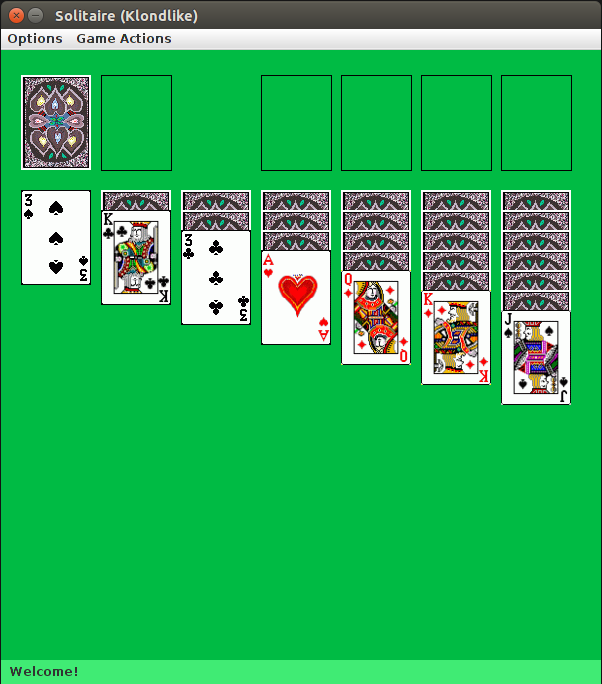
\includegraphics[width=9cm]{images/fig1.png}
		\caption{The opening window. The piles from left to right, top to
		bottom: Stock, Talon, 4 Foundations, 7 Tableus.}
		\label{fig:fig1}
	\end{figure}

	The play area makes up majority of the window, indicated by the green
	background.
	
	The menu bar contains the menu "Options", which include
	options to load a game from a save state, save the game, start a new game,
	or exit the game. It also contains the "Game Actions" menu, which allow
	the player to redeal cards or undo moves.

	The status bar at the bottom displays info such as the number of redeals
	the user has left, the number of stock cards, and a win message in case the
	user finishes the game.

	\newpage
	\section{Game Rules}
	\subsection{Starting Off}
	Much like in regular Klondlike Solitaire, the goal of the game is to get all
	the cards into the 4 foundation piles at the upper row. The cards are placed
	there by suit, with Aces at the bottom of the pile, and Kings at the top.

	The game starts off with most of the cards at the 7 tableus in the bottom
	row, with the first pile having 1 card, and the seventh having 7 cards. All
	the top cards of the tableus are always face up. The rest of the cards are
	in the stock pile, face down.

	\subsection{Moving Cards}
	To move cards, specifically among the talon, foundation, and tableu piles,
	just click on the card you want to move, then click on the pile you want to
	move them to. A black triangle indicator will indicate the clicked pile, as
	shown in Figure \ref{fig:fig2}.

	\begin{figure}[H]
		\centering
		\captionsetup{justification=centering}
		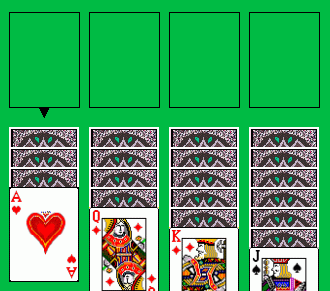
\includegraphics[width=9cm]{images/fig2.png}
		\caption{The black triangle indicator. In this case, the Ace card is
		clicked.}
		\label{fig:fig2}
	\end{figure}
	
	Do note that the indicator will not indicate which cards are clicked, just
	the pile of the clicked card.

	To move multiple cards, click on the base card of the pile of cards you want
	to move. For instance, if you want to move 3 cards, click the 3rd card from
	the top. Then, simply click the pile to which you want to move them.

	If you wish to cancel the movement, simply click elsewhere, like around the
	green play area. This will cancel the movement, as indicated by the loss of
	the indicator.

	\subsection{Card Placement}
	There exists a few rules when placing cards. These are the rules for moving
	to and from the stock / talon:
	\begin{itemize}
		\item You cannot get cards directly from the stock. You'll have to draw
		from the stock to the talon.
		\item Only one card can be thrown to or taken from the talon at a time.
	\end{itemize}

	These are the rules for moving to and from foundations:
	\begin{itemize}
		\item You can move only one card at a time to the foundations, even if
		all cards to be moved have valid placements in the foundations.
		\item When moving a card to the foundations, the card must be 1 rank
		higher than a card of similar suit in the foundations. Only Aces can
		be placed in the empty base.
		\item Sorting the foundation piles and cards by suit is done
		automatically. That is, you can move a valid card to any of the piles,
		given that a valid placement for that card exists in the foundation.
	\end{itemize}

	These are the rules for moving to and from tableus:
	\begin{itemize}
		\item You can only move cards that are faced up.
		\item You can move groups of 2 or more cards among tableus, granted that
		they are all face up.
		\item You can move a card / group of cards on a tableu if and only if:
		\begin{itemize}
			\item The base card is 1 rank lower than the card on top of the
			destination tableu. Only Kings can be moved onto empty tableus.
			\item The base card has to be of opposite color of the top card.
			\footnote{It follows that all face up cards in a tableu should be of
			alternating color.} For reference, Hearts and Diamonds are Red,
			while Spades and Clubs are Black.
		\end{itemize}
	\end{itemize}

	As an example, take note of Figure \ref{fig:fig3} below, which shows 4
	foundations and 4 tableus.

	\begin{figure}[H]
		\centering
		\captionsetup{justification=centering}
		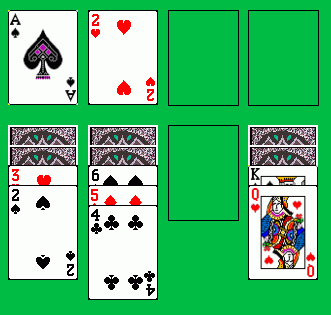
\includegraphics[width=9cm]{images/fig3.png}
		\caption{4 foundations and 4 tableus, for demonstration purposes.}
		\label{fig:fig3}
	\end{figure}

	By clicking on the 3 of Hearts in the first
	tableu, you can move it to the 2nd one by clicking on it, since the base
	card (3 of Hearts) is one rank lower than and of opposing color to the top
	card of the 2nd tableu (4 of Clubs). However, you can't move both the 3 of
	Hearts and the 2 of Spades at once to the foundations, even if both have
	valid positions in the foundations.

	You can also move the King and Queen on the 4th tableu to the empty 3rd one
	by clicking on the King first.

	When you accidentally make an invalid move, the program will ignore it, and
	nothing will happen.\footnote{Hopefully.}

	\subsection{Other Possible Moves}
	Aside from just moving cards around like that, you can also redeal the talon
	cards back to the stock. This is useful when you run out of stock cards,
	such as in Figure \ref{fig:fig4}. To do this, either click the empty stock
	pile, or go to the "Game Actions" menu and click "Redeal". Note that you
	only have a limited amount of redeals available. You always start with 2.

	\begin{figure}[H]
		\centering
		\captionsetup{justification=centering}
		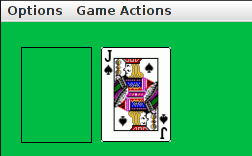
\includegraphics[width=9cm]{images/fig4.png}
		\caption{An empty stock with a talon stack.}
		\label{fig:fig4}
	\end{figure}

	You can also undo moves. To do so, go to "Game Actions" and click "Undo".
	Moves that can be undone include drawing, redealing, and moving cards
	between piles.\footnote{Note that when opening a save file (we'll get to
	that), the undo stack is lost, so you can't undo moves done before the save
	state was loaded.}

	\newpage
	\section{Save States}
	\subsection{Loading and Saving}
	A game can be loaded and saved. To save the current game, just go to
	"Options" and click "Save Game", then enter the filename to save the game on
	in the input prompt. To load a game, go to "Options" and then "Load Game",
	then enter the file name.

	\begin{figure}[H]
		\centering
		\captionsetup{justification=centering}
		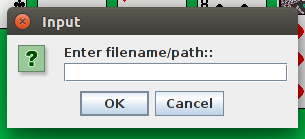
\includegraphics[width=9cm]{images/fig5.png}
		\caption{The prompt for the filename when loading or saving a file.}
		\label{fig:fig5}
	\end{figure}

	\subsection{Manually Editing a Save State}
	When a game is saved to a file, say, game.sltr, the data of the piles is
	written in a specific format which allows the app to read it back. An
	example of a save state is shown below, in Figure \ref{fig:fig6}.

	\begin{figure}[H]
		\centering
		\captionsetup{justification=centering}
		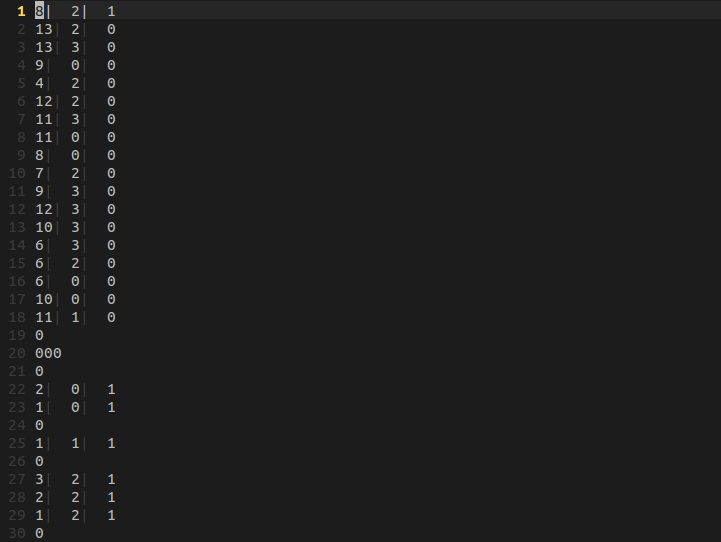
\includegraphics[width=9cm]{images/fig6.png}
		\caption{A game save state. Note that this isn't the entire save state,
		just the stock, talon, and first foundation.}
		\label{fig:fig6}
	\end{figure}

	The data can be interpreted as such:
	\begin{verbatim}
	<stock pile>
	0
	<talon pile>
	0
	<foundation pile 1>
	0
	...
	0
	<tableu pile 1>
	0
	...
	0
	<tableu pile 7>
	0
	\end{verbatim}
	Notice how each pile is separated by a 0.

	Each pile is represented as a list of cards, with each line representing
	a card, and the first line representing the top card. The following is an
	example of a card representation:
	\begin{verbatim}
	3	1	0
	\end{verbatim}

	The first digit represent the rank. The second represent the suit. In this
	case, a 0 means Spades, a 1 means Hearts, a 2 means Diamonds, and a 3 means
	Clubs. The third represents whether or not the card is face up. A one
	represents a face-up card, and vice-versa. In the case above, the card is
	a face-down 3 of Hearts.

	It's important to note that the digits are separated by hard tabs, or
	\verb|\t|, not a bunch of spaces. Soft tabs are considered a bunch of
	spaces, so keep that in mind.

	If the pile is empty, then it is represented by three non-separated 0s, as
	shown below:
	\begin{verbatim}
	000
	\end{verbatim}

	Finally, note that the save state isn't validated upon loading, so creating
	impossible scenerios such as the one in Figure \ref{fig:fig7} is possible.
	\footnote{Do note that the win condition is based solely on the total number
	of cards in the foundation.}

	\begin{figure}[H]
		\centering
		\captionsetup{justification=centering}
		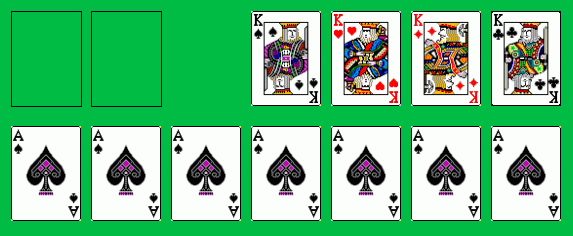
\includegraphics[width=9cm]{images/fig7.png}
		\caption{An impossible game.}
		\label{fig:fig7}
	\end{figure}
\end{document}
